\scanpage{40}
\uline{II.} Caractérisation des op. de Fredholm : $u\in L^{(1)}(E,F)\Longleftrightarrow\sum\rho_i(u)<+\infty$; et alors on a
\[
\boxed{\|u\|_1=\sum\rho_i(u)}.
\]
\unsure{Corollaire 1} $u$ Fredholm $\Longleftrightarrow |u|$ Fredholm, et $\|u\|_1=\||u|\|_1=\operatorname{Tr}|u|$.

\uline{\unsure{Corollaire 2}} On a alors $|\operatorname{Tr}u|\leq\sum\rho_i(u)$.
\margin{Notation $L^{(1)}(E,F)$ et $E\widehat\otimes^{(1)}F$}
\margin{$n\leq\dim E,\ \dim F$ \uline{\unsure{Théorie de Riesz}}}

\uline{\unsure{Remarque 2}} Si $u\in L_0(E,E')$ :
\[
\boxed{\sum_1^n\rho_i(u)=\deleted{\unsure{\sum}}\sup|\operatorname{Tr}v_nu|}\qquad
\begin{gathered}
v_n\in L(E',E)\\
\|v_n\|\leq1\\
\operatorname{rang}v_n\leq n
\end{gathered}
\]
\deleted{\unsure{$v_n$ projecteur} \unsure{orthogonal}}
où le sup est atteint aux \deleted{\unsure{projections orthogonales de rang} $n$} \unsure{où} \unsure{$v_n$ est} \inserted{$v_n=p_nv_n$ ($p_n$ \unsure{projection|projecteur} \unsure{hermitien} de rang $n$)} \unsure{si} $\unsure{u}$ est \unsure{hermitien}. \deleted{dans $E$} \inserted{de dim $E\geq n$}.

\deleted{En effet on a
\[
\operatorname{Tr}p_nu=\operatorname{Tr}p_n^2u=\operatorname{Tr}p_nup_n,
\]
\unsure{soit} $w$ la restriction de $p_nup_n$ à $p_n(E)$, on a
\[
\deleted{\unsure{|\operatorname{Tr}p_nup_n|=}}\quad
|\operatorname{Tr}p_nu|=|\operatorname{Tr}w|\leq\deleted{\unsure{\dim E}}\sum_1^n\rho_i(w),
\]
or
\[
\rho_i(w)=\rho_i(p_nup_n)\leq\rho_i(up_n)\leq\rho_i(u),
\]
d'où $|\operatorname{Tr}p_nu|\leq\sum_1^n\rho_i(u)$.}

\deleted{D'où $|\operatorname{Tr}v_nu|\leq\sum_1^n\rho_i(u)$, et si $u=\sum_1^\infty\rho_i\overline e_i\otimes f_i$;}
\deleted{\unsure{Réciproquement}} \deleted{\unsure{En effet}}
\inserted{car $\rho_i(uv_n)\leq\rho_i(u)\|v_n\|=\rho_i(u)$.}
\deleted{\unsure{On peut} prouver $|\operatorname{Tr}v_nu|\leq\sum_1^n\rho_i(u)$, \unsure{il suffit de} l'inégalité}

\deleted{\unsure{Soit} $w$ un op. \inserted{de rang $\leq n$}, et $w=p_nw$, $p_n$ un projecteur de rang $n$, et $\operatorname{Tr}w=\operatorname{Tr}p_nw=\operatorname{Tr}p_n^2w=\operatorname{Tr}\figure{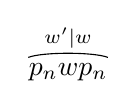
\begin{tikzpicture}[baseline=(pnwpn.base)]
\node[inner sep=0pt] (pnwpn) {$p_nwp_n$};
\draw[line width=0.4pt] ([yshift=2pt]pnwpn.north west) .. controls ([xshift=5pt,yshift=4pt]pnwpn.north west) and ([xshift=-5pt,yshift=4pt]pnwpn.north east) .. ([yshift=2pt]pnwpn.north east);
\node[anchor=south,inner sep=0pt] at ([yshift=5pt]pnwpn.north) {$\scriptstyle\inserted{\unsure{w'|w}}$};
\end{tikzpicture}}$. \unsure{On soit|On sait si} $w'$ la restriction \unsure{de} $p_nwp_n$ à $p_n(E)$, on obtient
\[
\unsure{|\operatorname{Tr}w|=}\quad|\operatorname{Tr}w'|\leq\sum_1^n\rho_i(w'),
\]
$\unsure{w'=}$
\[
\rho_i(w')=\deleted{\unsure{\rho_i(p_nwp_n)}}\deleted{\unsure{\|p_n\|}}=\rho_i(wp_n)\leq\rho_i(w),
\]
$\boxed{\rho_i(w')\leq\rho_i(w)}$, \deleted{\unsure{w sur un espace de}} \unsure{d'où l'inégalité} $\unsure{\sum\rho_i(w)}$.}

\margin{$|\operatorname{Tr}v_nu|\leq\sum_1^n\rho_i(u)$ \unsure{est une} \inserted{conséquence} \unsure{du} \uline{lemme} Si $w$ est un opérateur \unsure{\deleted{linéaire}|linéaire} de rang $\leq n$ de $E$ dans lui,
\[
|\operatorname{Tr}w|\leq\sum_1^n\rho_i(w).
\]
En effet, soit $v$ la restriction de $w$ à $w(E)$, alors on a $|\operatorname{Tr}w|=|\operatorname{Tr}v|\leq\sum_1^n\rho_i(\unsure{w|v})$ $(\unsure{\text{---}})$.
Or $v=\alpha^*w\alpha$, où $\alpha$ est l'injection \unsure{canonique} de $w(E)$ dans $E$, d'où $\rho_i(v)\leq\|\alpha^*\|\|\alpha\|\rho_i(w)\leq\rho_i(w)$, d'où $|\operatorname{Tr}w|\leq\sum_1^n\rho_i(w)$.}

Pour prouver que la borne est \inserted{atteinte} \deleted{\unsure{obtenue}}, on écrit $u=\sum_1^{\unsure{n|\infty}}\rho_i\overline e_i\otimes f_i$, et on prend
\[
v_n=\sum_{j=1}^n\overline{\unsure{f_j|f_i}}\otimes\unsure{e_j|e_i},
\]
\margin{\figure{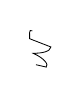
\begin{tikzpicture}[x=0.5cm,y=0.5cm]
\draw[line width=0.3pt] (0.18,1.00) .. controls (0.07,1.07) and (0.12,0.87) .. (0.11,0.80) -- (0.65,0.59) .. controls (0.63,0.47) and (0.42,0.43) .. (0.20,0.43) .. controls (0.49,0.30) and (0.60,0.14) .. (0.53,0.08) -- (0.27,0.14);
\end{tikzpicture}}}
on a \deleted{\unsure{alors}}
\[
v_nu=\sum_{\substack{ij\\j\leq n}}\rho_i\overline e_i\otimes e_j\,(f_i,f_j)
=\sum_{j\leq n}\rho_{\unsure{i|j}}\overline e_{\unsure{i|j}}\otimes\unsure{e_j|e_i},
\]
dont la trace est $\sum_1^n\rho_i$, $v_n$ est un projecteur hermitien si $u$ était supposé hermitien $(f_i=e_i)$.
\margin{(?)}
\unsure{Comme les particuliers en un corollaire, on a}

\uline{Corollaire \unsure{4|3}} Soient $u,v\in L_0(E,F)$, alors
\[
\boxed{\sum_1^n\rho_i(u+v)\leq\sum_1^n\bigl(\rho_i(u)\unsure{-|+}\rho_i(v)\bigr)}.
\]
Cas particulier $\|u+v\|_1\leq\|u\|_1+\|v\|_1$.
On peut aussi dire que $\sum_{i=1}^n\rho_i$ est une ``\uline{norme}'' sur $L_0(E,F)$.

\margin{\figure{\begin{tikzpicture}[x=0.6cm,y=0.6cm]
\draw[line width=0.3pt] (0,0.08) .. controls (0.30,-0.02) and (0.66,0.01) .. (0.79,0.26) .. controls (0.93,0.07) and (1.19,0.03) .. (1.40,0.13);
\fill (1.55,0.18) circle (0.015);
\end{tikzpicture}}}

\uline{\unsure{Dém}}
\mspage{41}
